\chapter{Background}
\label{ch:background}

This chapter fixes the vocabulary and the notation that the rest of the
thesis uses. It defines the basic objects of a trading venue --- orders,
the limit order book, trades --- and then gives a precise description of
the two matching mechanisms compared in this thesis, the continuous double
auction (CDA) and the frequent batch auction (FBA). It closes with the
formal definition of every metric used in the empirical comparison of
\Cref{ch:results}. Why these mechanisms and these metrics matter is the
subject of \Cref{ch:foundations}; this chapter only says precisely what
they are.

\section{Basic Terminology and Notation}
\label{sec:terminology}

\subsection{Orders}

A venue trades one \emph{asset pair}, here SOL against USD. Prices $p$ are
quoted in USD per SOL and quantities $q$ in SOL. An \emph{order} $k$ is an
instruction to buy or sell and is described by
\begin{equation}
  k = (s_k,\; q_k,\; \pi_k,\; t_k),
\end{equation}
where $s_k \in \{\text{buy}, \text{sell}\}$ is its side, $q_k > 0$ its
quantity, $\pi_k$ its limit price and $t_k$ its submission time. A buy
order is also called a \emph{bid} and a sell order an \emph{ask}; the sets
of bids and asks in a given collection of orders are written $\mathbb{B}$
and $\mathbb{A}$.

A \emph{limit order} trades only at its limit price or better: a bid at
$\pi_k$ or lower, an ask at $\pi_k$ or higher. A \emph{market order} has no
limit and accepts any price; it is treated as a bid with no upper price
limit or an ask with no lower price limit. A \emph{cancellation} removes a
previously submitted order that has not yet been filled. An order's
\emph{time-in-force} states how long it may wait to be filled (for example
until cancelled, or immediately or never); \Cref{sec:environment} states
which of these rules the simulated engines enforce.

\subsection{The Limit Order Book}

A \emph{limit order book} is the set of limit orders that have been
submitted, not yet filled and not cancelled. These orders are said to
\emph{rest} in the book. Orders with the same limit price form a
\emph{price level}. At time $t$ the \emph{best bid} $b_t$ is the highest
resting bid price and the \emph{best ask} $a_t$ the lowest resting ask
price. Their midpoint and the quoted spread are
\begin{equation}
  \label{eq:midpoint}
  \midp = \frac{a_t + b_t}{2},
  \qquad
  \text{quoted spread}_t = a_t - b_t .
\end{equation}
The quantity resting at a price level is the \emph{depth} at that level;
the quantity at $b_t$ and $a_t$ is the depth \emph{at the best}, or at
the \emph{touch}. Relative quantities are expressed in \emph{basis points}
(bps), $1\,\text{bps} = 10^{-4}$, so that a price $p$ lies
$|p - m|/m \cdot 10^{4}$\,bps away from a reference price $m$.

\subsection{Trades, Makers and Takers}

A \emph{trade} is an exchange of quantity between one buy order and one
sell order at one price. When an arriving order is matched against a
resting order, the resting order is the \emph{maker} (it supplied
liquidity) and the arriving order the \emph{taker} or \emph{aggressor} (it
demanded liquidity). A trade is indexed like an order: trade $k$ has price
$p_k$, quantity $q_k$ and time $t_k$, and whether $k$ denotes an order or a
trade is always clear from context. The direction of trade $k$ is
$\varepsilon_k = +1$ if the aggressor was a buyer and $\varepsilon_k = -1$
if it was a seller. The signed quantity $\varepsilon_k q_k$, summed over a
set of trades, is their net \emph{order flow}: positive when buying
pressure dominates. A participant who quotes on both sides of the book to
earn the spread is a \emph{market maker} or \emph{liquidity provider}.

\Cref{tab:notation} collects every symbol used in the thesis, grouped by
topic, with the section in which each is defined.

\begingroup
\small
\renewcommand{\arraystretch}{1.15}
\begin{longtable}{@{}p{3.3cm} p{10.4cm} p{2.0cm}@{}}
\caption[Notation]{Notation used throughout the thesis.}
\label{tab:notation}\\
\toprule
\textbf{Symbol} & \textbf{Meaning} & \textbf{Defined in}\\
\midrule
\endfirsthead
\multicolumn{3}{@{}l}{\emph{\Cref{tab:notation}, continued}}\\
\toprule
\textbf{Symbol} & \textbf{Meaning} & \textbf{Defined in}\\
\midrule
\endhead
\bottomrule
\endfoot
\multicolumn{3}{@{}l}{\emph{Orders, book and trades}}\\
$p,\ q$ & a price (USD per SOL) and a quantity (SOL) & \S\ref{sec:terminology}\\
$k$ & index of an order, or of a trade & \S\ref{sec:terminology}\\
$s_k, q_k, \pi_k, t_k$ & side, quantity, limit price and submission time of order $k$ & \S\ref{sec:terminology}\\
$j$ & a resting order that an arriving order trades against (CDA) & \S\ref{sec:cdaformal}\\
$\mathbb{B}, \mathbb{A}$ & sets of bids (buy orders) and asks (sell orders) of a batch or a book & \S\ref{sec:terminology}\\
$b_t, a_t$ & best bid and best ask of the CDA book at time $t$ & \S\ref{sec:terminology}\\
$\midp$ & midpoint $(a_t + b_t)/2$ of the CDA book at time $t$ & \eqref{eq:midpoint}\\
$m$ & a reference price against which a distance in bps is measured & \S\ref{sec:terminology}\\
$p_k, q_k, t_k$ & price, quantity and time of trade $k$ & \S\ref{sec:terminology}\\
$\varepsilon_k$ & direction of trade $k$: $+1$ buyer-initiated, $-1$ seller-initiated & \S\ref{sec:terminology}\\
\midrule
\multicolumn{3}{@{}l}{\emph{Batch clearing}}\\
$\tau$ & batch interval of the FBA; also the width of a measurement bucket ($\tau = 1$\,s in the run) & \S\ref{sec:fbanotation}\\
$\mathbf{1}\{\cdot\}$ & indicator function: $1$ if the condition holds, $0$ otherwise & \eqref{eq:demandsupply}\\
$D(p), S(p)$ & cumulative demand and supply of a batch at price $p$ & \eqref{eq:demandsupply}\\
$V(p)$ & executable volume $\min\{D(p), S(p)\}$ at price $p$ & \S\ref{sec:fbanotation}\\
$\mathcal{P}^{*}$ & set of volume-maximising prices & \S\ref{sec:fbanotation}\\
$\underline{p}, \overline{p}$ & lowest and highest price in $\mathcal{P}^{*}$ & \S\ref{sec:fbanotation}\\
$V^{*}$ & maximal executable volume of a batch & \S\ref{sec:fbanotation}\\
$\sigma$ & tie-break rule selecting one price from $\mathcal{P}^{*}$ & \eqref{eq:clearing}\\
$\clr$ & clearing price of a batch, $\clr = \sigma(\mathcal{P}^{*})$ & \eqref{eq:clearing}\\
$p_{\mathrm{prev}}$ & clearing price of the previous batch that traded (tie-break step 3) & \S\ref{sec:fbanotation}\\
$x_k$ & quantity of order $k$ executed in a batch & \S\ref{sec:fbanotation}\\
\midrule
\multicolumn{3}{@{}l}{\emph{Surplus}}\\
$W^{\mathbb{B}}(p), W^{\mathbb{A}}(p)$ & buyer and seller surplus (price improvement against own limits) of a batch at price $p$ & \eqref{eq:surplus}\\
$W$ & total surplus of a batch, $W = W^{\mathbb{B}}(\clr) + W^{\mathbb{A}}(\clr)$; independent of the price chosen in $\mathcal{P}^{*}$ & \eqref{eq:surplus}, \eqref{lem:invariance}\\
\midrule
\multicolumn{3}{@{}l}{\emph{Measurement grid}}\\
$t_0$ & timestamp of the first record of the run & \eqref{eq:bucket}\\
$\mathrm{bucket}(t)$ & the one-second bucket containing time $t$ & \eqref{eq:bucket}\\
$e$ & engine, $e \in \{\mathrm{CDA}, \mathrm{FBA}\}$ & \S\ref{sec:measurement}\\
$M^{e}_t$ & value of metric $M$ for engine $e$ in bucket $t$ & \S\ref{sec:measurement}\\
$d_t$ & paired difference $M^{\mathrm{FBA}}_t - M^{\mathrm{CDA}}_t$ & \S\ref{sec:measurement}\\
$n$ & number of buckets (or days) with a paired value & \S\ref{sec:experiments}\\
\midrule
\multicolumn{3}{@{}l}{\emph{Metrics}}\\
$h$ & distance threshold of depth within $h$ bps, $h \in \{10, 50, 100\}$ & \S\ref{sec:metrics21}\\
$m_k$ & pre-trade reference price of trade $k$ & \S\ref{sec:metrics21}\\
$\Delta$ & markout horizon, $\Delta \in \{1, 5, 30\}$\,s & \S\ref{sec:metrics21}\\
$m_{k+\Delta}$ & first reference price at or after $t_k + \Delta$ & \S\ref{sec:metrics21}\\
$S^{\mathrm{eff}}_k$ & effective spread of trade $k$ & \eqref{eq:effspread}\\
$S^{\mathrm{real}}_k(\Delta)$ & realized spread of trade $k$ at horizon $\Delta$ & \eqref{eq:realspread}\\
$\mathrm{PI}_k(\Delta)$ & price impact of trade $k$ at horizon $\Delta$ & \eqref{eq:priceimpact}\\
$r_i$ & $i$-th consecutive return of the reference price within a bucket & \S\ref{sec:formularq22}\\
$\mathcal{T}$ & set of buckets in which both engines traded & \S\ref{sec:formularq22}\\
$\mathrm{VWAP}^{e}_t$ & volume-weighted average price of engine $e$ in bucket $t$ & \S\ref{sec:formularq22}\\
$r^{e}_i$ & log return of $\mathrm{VWAP}^{e}$ between consecutive buckets of $\mathcal{T}$ & \eqref{eq:matchedvol}\\
$\mathrm{vol}^{e}_{\text{day}}$ & matched-timestamp volatility of engine $e$ on one day & \eqref{eq:matchedvol}\\
$\lambda$ & Kyle's lambda, price change per unit of net order flow & \S\ref{sec:formularq22}\\
$f_i, y_i$ & net signed order flow and price change (bps) of observation $i$ in the Kyle regression & \S\ref{sec:formularq22}\\
$m_{\mathrm{pre}}, m_{\mathrm{post}}$ & CDA midpoint before a sweep and 5\,s after it & \S\ref{sec:formularq22}\\
$\mu$ & prior expected value of the asset in the model of \citet{kyle1985continuous} & \S\ref{sec:adverse}\\
\midrule
\multicolumn{3}{@{}l}{\emph{Design analysis}}\\
$\delta$ & difference in message latency between two participants & \S\ref{sec:interval}\\
$\tau_{\min}, \tau_{\max}$ & bounds of a randomised closing time & \S\ref{sec:interval}\\
$i$ & a participant (in sums: an observation index) & \S\ref{sec:priceimprovement}\\
$\ell_i$ & message latency of participant $i$ & \eqref{prop:latency}\\
$\kappa$ & share of the marginal volume allocated pro rata in a hybrid rationing rule & \S\ref{sec:rationing}\\
\end{longtable}
\endgroup

\section{The Continuous Double Auction}
\label{sec:cdaformal}

The CDA processes orders one at a time, in the order the venue receives
them, against a limit order book. Resting orders are ranked by
\emph{price-time priority}: a better price first, and among orders at the
same price, the earlier one first. When a buy order $k$ arrives, it is
matched as follows (a sell order is symmetric, with bids in place of
asks):
\begin{enumerate}
  \item While $k$ has quantity left and the book holds an ask with
  $a_t \le \pi_k$ (always, for a market order), $k$ trades against the
  first-ranked order $j$ at the best ask. The trade price is the
  \emph{resting} order's price, $p = a_t$, and the trade quantity is
  $\min(q_k, q_j)$; both remaining quantities are reduced by it, and a
  fully filled resting order leaves the book.
  \item Any quantity of a limit order that is left when no further ask
  crosses rests in the book at $\pi_k$, behind the orders already resting
  at that price. The unfilled remainder of a market order does not rest.
\end{enumerate}
Three properties of this rule matter for the comparison. Execution is
immediate: an order that can trade does so the instant it arrives. A
single order that sweeps several price levels trades at several prices.
And the maker--taker distinction is defined by arrival order, so every
CDA trade has a known aggressor and direction $\varepsilon_k$.

\section{The Frequent Batch Auction}
\label{sec:fbanotation}

A frequent batch auction collects orders over a half-open window $[0,\tau)$
of length $\tau$ and, at the end of the window, considers all of them
together instead of one at a time. Let $\mathbb{B}$ and $\mathbb{A}$
denote the sets of bids and asks in the batch. A market bid is treated as
having no upper price limit and a market ask as having no lower price
limit, so it never falls out of either schedule below on grounds of
price.

\subsection{Demand and Supply}

The batch is cleared the same way an economics textbook clears a market: by
lining up how much would be bought against how much would be sold at every
possible price, and finding where the two balance. For any price $p$, the
bid side gives the cumulative \emph{demand} at that price and the ask side
gives the cumulative \emph{supply}, exactly as in that textbook picture.
Demand is the quantity buyers are willing to take at $p$ or less, so it can
only fall as $p$ rises: a bid counts toward it once its limit price is at
least $p$, and drops out as soon as $p$ climbs past that limit. Supply is
the mirror image: the quantity sellers are willing to give up at $p$ or
more, which can only rise as $p$ rises, since an ask counts once its limit
price is at most $p$. Written out, with the market-order convention above,
\begin{equation}
  \label{eq:demandsupply}
  D(p) = \sum_{k \in \mathbb{B}} q_k \mathbf{1}\{\pi_k \ge p\},
  \qquad
  S(p) = \sum_{k \in \mathbb{A}} q_k \mathbf{1}\{\pi_k \le p\}.
\end{equation}
Plotted against price, $D$ and $S$ are \emph{step} curves rather than
smooth ones, because each order adds its whole quantity at once, the
moment its limit price is reached, rather than a little at a time: $D$
steps down as price rises, $S$ steps up. \Cref{fig:fbaschedule} shows
exactly this picture for a small worked example. At any price $p$, only
the smaller of the two sides can actually trade, so the volume executable
at that price is
\begin{equation}
  V(p) = \min\{D(p), S(p)\}.
\end{equation}

\begin{figure}[htbp]
\centering
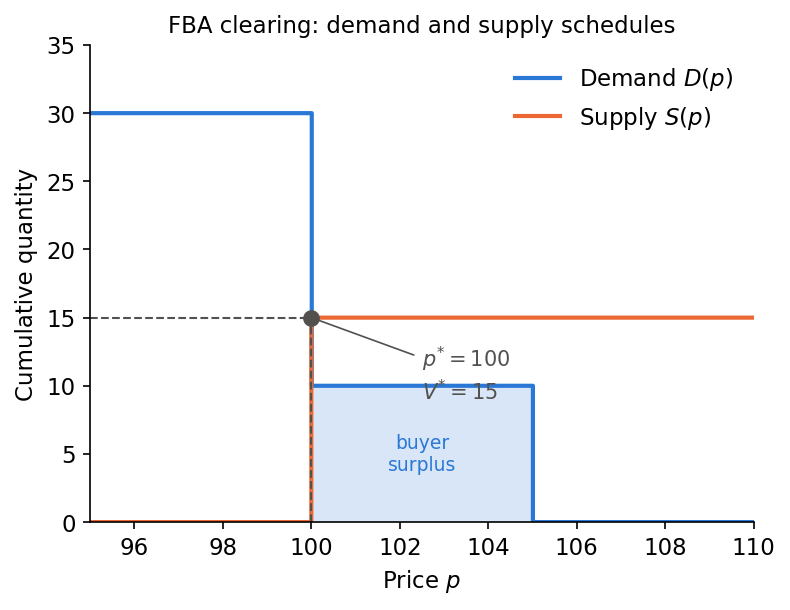
\includegraphics[width=0.72\textwidth]{figures/fig_fba_schedule.png}
\caption[FBA clearing as a supply/demand diagram]{The FBA clearing
mechanism drawn as a classical demand/supply diagram: $D(p)$ and $S(p)$
as step functions of price. Reading it: pick any price on the horizontal
axis; the height of the demand step there is how much would be bought at
that price or cheaper, the height of the supply step is how much would be
sold at that price or dearer. The two curves bind, i.e.\ reach their
largest common height, at the clearing price $\clr$, marked where they
meet. Drawn from a small illustrative example (four orders, three buys
and one sell), chosen because it clears without a tie and so needs no
tie-break cascade (below) to illustrate the basic mechanism cleanly; a
real batch from the simulated month has dozens of orders and does not
render legibly at this scale.}
\label{fig:fbaschedule}
\end{figure}

\subsection{Finding the Clearing Price}

The two curves do not have to cross at one exact price: they can run side
by side, both holding the same height, across several price ticks at
once, which happens often when the book is thin. Every price in that
stretch executes the same maximum volume, so volume by itself cannot say
which one is actually used. The clearing rule therefore works in two
stages. First, it finds every price that reaches the greatest executable
volume, the volume-maximising set
\begin{equation}
  \mathcal{P}^{*} = \argmax_{p \in \mathbb{R}_{+}} V(p),
  \qquad V^{*} = \max_{p} V(p),
\end{equation}
which, since $D$ is non-increasing and $S$ is non-decreasing, is a single
closed interval $[\underline{p}, \overline{p}]$ whenever the book crosses
at all ($V^{*} > 0$). When that interval holds more than one price, a
second, tie-breaking stage is needed to pick exactly one of them:
\begin{equation}
  \label{eq:clearing}
  \clr = \sigma\bigl(\mathcal{P}^{*}\bigr) \in \mathcal{P}^{*}.
\end{equation}
Real auctions resolve this indeterminacy with a fixed cascade of
tie-breaking steps, applied in order until one price remains
\citep{haynes2020precedence}, and the engine used in this thesis follows
exactly this cascade (\Cref{app:config}):
\begin{enumerate}
  \item choose the price (or prices) that maximise $V(p)$ --- this is
  $\mathcal{P}^{*}$ itself;
  \item if $\mathcal{P}^{*}$ is not a singleton, choose the price that
  minimises the residual imbalance $|D(p) - S(p)|$;
  \item if still tied, choose the price closest to the auction's own
  previous clearing price $p_{\mathrm{prev}}$;
  \item if still tied, choose the lowest such price.
\end{enumerate}

\subsection{Allocation, Rationing and the Residual}

Let $x_k \ge 0$ denote the executed quantity of order $k$ under a
volume-maximising allocation, so that $\sum_{k \in \mathbb{B}} x_k =
\sum_{k \in \mathbb{A}} x_k = V^{*}$. Every trade of the batch is at the
single price $\clr$. At $\clr$ the two sides are usually not equal,
$D(\clr) \ne S(\clr)$, so the orders on the longer side cannot all be
filled and a \emph{rationing rule} decides which are. The engine used here
ranks the eligible orders of each side by \emph{price-time priority within
the batch}: market orders first, then the better limit price, then the
earlier submission, and fills them in that order until the shorter side
is used up (\Cref{sec:rationing} discusses the alternatives). The volume
left unmatched, $|D(\clr) - S(\clr)|$ on the longer side together with
every order that was not eligible at $\clr$, is the \emph{residual}; in
this thesis it rolls over into the next batch unchanged.

\subsection{Price Improvement and Surplus}

Uniform pricing gives every executed order a price at least as good as
the one it asked for, and every inframarginal order a strictly better
one; \Cref{fig:fbaschedule} shows exactly how much better. A buyer
with limit price $\pi_k$ above $\clr$ does not pay $\pi_k$; the whole
batch pays $\clr$, so this order keeps the gap $\pi_k - \clr$ for every
unit it trades. In \Cref{fig:fbaschedule} this gap is the shaded
rectangle: its width is how far that order's limit sits above the
clearing price, its height is how much of it trades, and its area is
what that order gains by not having to pay what it was willing to.
Sellers gain the mirror amount, $\clr - \pi_k$, the gap between the
clearing price and their own limit. Summed over every executed order,
these gaps are the familiar consumer- and producer-surplus areas from an
introductory supply/demand diagram, just read off a single discrete
batch instead of a continuous market: the buyers' share sits above
$\clr$, under the demand curve; the sellers' share sits below $\clr$,
above the supply curve.

Formally, each side's surplus at a candidate price $p$ is
\begin{equation}
  \label{eq:surplus}
  W^{\mathbb{B}}(p) = \sum_{k \in \mathbb{B}} (\pi_k - p)\, x_k,
  \qquad
  W^{\mathbb{A}}(p) = \sum_{k \in \mathbb{A}} (p - \pi_k)\, x_k,
\end{equation}
and total surplus at the batch's own clearing price is $W =
W^{\mathbb{B}}(\clr) + W^{\mathbb{A}}(\clr)$. Every
term in both sums is non-negative for an executed order --- a buy only
has $x_k>0$ if $\pi_k \ge \clr$, and a sell only if $\pi_k \le \clr$, so
no order ever executes at a loss relative to its own limit. This is what
\Cref{ch:results} measures as \emph{trader surplus}. The worked example
also previews a point \Cref{sec:priceimprovement} returns to in full: the
two sides need not split $W$ evenly, or even at all. Here the entire
gain goes to the buyers, because the seller's own limit happens to equal
the clearing price. In this example $\mathcal{P}^{*}$ holds the single
price $100$, so the split is pinned down; when $\mathcal{P}^{*}$ holds
several prices, choosing a different one would split $W$ differently
without changing who trades or how much.

\subsection{What Differs from the CDA}

Set against \Cref{sec:cdaformal}, the FBA changes three things. Orders
wait up to $\tau$ before they can trade, instead of trading on arrival.
All trades of a batch share one price $\clr$, instead of each trading at
the resting order's price. And because the orders of a batch trade
simultaneously, no order crosses another's quote: there is no maker and
no taker, and a trade has no observable direction $\varepsilon_k$. This last point
is the reason several metrics below need an adaptation for the FBA.

\section{Measurement Framework}
\label{sec:measurement}

Both engines are measured on one common time grid. Every observation is
assigned to a fixed-width time \emph{bucket},
\begin{equation}
  \label{eq:bucket}
  \mathrm{bucket}(t) = t_0 + \left\lfloor \frac{t - t_0}{\tau} \right\rfloor \tau,
\end{equation}
where $t_0$ is the timestamp of the first record of the run and the
width equals the batch interval, $\tau = 1$\,second throughout this
thesis. Every metric below is computed once per bucket and per engine, so
each bucket yields one CDA value and one FBA value from the same order
flow. Buckets are contiguous: a bucket with no qualifying observation
still exists, with the metric marked missing. A missing value (``no
qualifying observation in this bucket'') and a value of zero (``there were
observations and the value is zero'') are kept distinct.

For a metric $M$ computable on both engines, the comparison is the
\emph{paired difference} $d_t = M^{\mathrm{FBA}}_t - M^{\mathrm{CDA}}_t$
over the buckets in which both values exist; \Cref{sec:experiments}
describes how its standard error is estimated. A metric that exists for
only one engine is reported descriptively.

\section{Metrics}
\label{sec:metricdefs}

Each metric below is tagged with its \emph{scope}: \textbf{U} (computed for
both engines) or \textbf{F} (FBA only). The metrics are grouped by
the part of RQ2 (\Cref{sec:rqs}) they answer. \Cref{tab:metrics} gives an
overview; \Cref{ch:foundations} explains why each is used.

\begin{table}[htbp]
\centering
\caption[Overview of the metrics]{Overview of the metrics, by research
question. Scope: U both engines, F FBA only.}
\label{tab:metrics}
\small
\begin{tabularx}{\textwidth}{@{}l l L c@{}}
\toprule
\textbf{RQ} & \textbf{Metric} & \textbf{What it measures} & \textbf{Scope}\\
\midrule
2.1 & Quoted spread & cost of crossing the book now & U\\
    & Depth at best / within $h$ bps & quantity available near the price & U\\
    & Effective spread & cost an actual trade paid & U\\
    & Realized spread & part of that cost the maker keeps & U\\
    & Price impact & part lost to informed traders & U\\
    & Amihud illiquidity & price move per dollar traded & U\\
\midrule
2.2 & Matched-timestamp volatility & price variability on a common grid & U\\
    & Intra-interval dispersion & price variation within one second & U\\
    & Kyle's lambda & price move per unit of order flow & U\\
\midrule
2.3 & Executed volume, trade count & how much trades & U\\
    & Time to execution & how long orders wait & U\\
    & Trader surplus & price improvement against the limit & U\\
    & Boundary concentration & arrivals near the batch close & F\\
    & Unexecuted residual share & imbalance left at $\clr$ & F\\
\midrule
--- & Throughput, clearing latency & computing speed (control) & U\\
\bottomrule
\end{tabularx}
\end{table}

\subsection{Liquidity and Transaction Costs (RQ2.1)}
\label{sec:metrics21}

\paragraph{Quoted spread (U).} For the CDA, every book snapshot in the
bucket with both sides present contributes $(a_t - b_t)/\midp \cdot
10^{4}$\,bps, and the bucket value is the mean over snapshots. The FBA
has no book while a batch accumulates; its analogue is the gap between the
best unfilled sell and the best unfilled buy among the orders left after
a clear (including those rolled over from earlier batches), relative to
$\clr$ and in bps, averaged over the batches in which both exist.

\paragraph{Depth at best (U).} For the CDA, the mean over snapshots of
(best-bid size $+$ best-ask size)$/2$, the touch only. For the FBA, the
mean over batches of $(D(\clr) + S(\clr))/2$, the quantity eligible to
trade at the clearing price.

\paragraph{Depth within $h$ bps (U), $h \in \{10, 50, 100\}$.} The
quantity of all orders priced within $h$\,bps of a reference price, half
the sum of both sides, cumulative across thresholds. The orders counted
are those in the book (CDA, reference $\midp$) or pending in the batch
just before it clears (FBA, rolled-over orders included, reference
$\clr$).

\paragraph{Effective, realized spread and price impact (U).} Let trade
$k$ have price $p_k$, direction $\varepsilon_k$, pre-trade reference price $m_k$
and, a markout horizon $\Delta$ later, reference price $m_{k+\Delta}$.
In proportional form \citep{hasbrouck1993assessing,hendershott2011algorithmic},
\begin{align}
  S^{\mathrm{eff}}_k &= \frac{2 \varepsilon_k (p_k - m_k)}{m_k},
    \label{eq:effspread}\\[3pt]
  S^{\mathrm{real}}_k(\Delta) &= \frac{2 \varepsilon_k (p_k - m_{k+\Delta})}{m_k},
    \label{eq:realspread}\\[3pt]
  \mathrm{PI}_k(\Delta) &= \frac{2 \varepsilon_k (m_{k+\Delta} - m_k)}{m_k},
    \label{eq:priceimpact}
\end{align}
each in bps after multiplying by $10^{4}$, so that $S^{\mathrm{eff}}_k =
S^{\mathrm{real}}_k(\Delta) + \mathrm{PI}_k(\Delta)$ trade by trade and in
any quantity-weighted aggregate. The bucket value is the
quantity-weighted mean over the bucket's trades, for $\Delta \in
\{1, 5, 30\}$\,s. For the CDA, $m_k$ is the book midpoint before the trade
and $m_{k+\Delta}$ the first midpoint at or after $t_k + \Delta$. The FBA
needs two adaptations. Its reference price $m_k$ is the previous batch's
clearing price as of the order's submission, since there is no midpoint
while a batch accumulates, and $m_{k+\Delta}$ is the first FBA clearing
price at or after $t_k + \Delta$. And its trades have no direction $\varepsilon_k$
(\Cref{sec:fbanotation}), so the simulator records only the unsigned
deviation $2|p_k - m_k|/m_k$.

\paragraph{Signing the FBA side.} Before the FBA values are compared, each
bucket in which both engines traded is given a direction by a zero-tick
rule \citep{leeready1991} applied to \emph{consecutive CDA prices}: the
second's FBA trades are labelled buys if the CDA price ticked up, sells if
it ticked down, and inherit the last nonzero tick otherwise. The reported
FBA effective and realized spread are this sign times the unsigned
values, and the FBA price impact is the signed effective spread minus the
signed realized spread. Signing with the FBA's own price history instead
would be circular, because that history is $m_k$ itself, so the sign
would only undo the deviation's own sign. The rule is an estimate, not
an observed direction; \Cref{sec:res21} discusses what it can and cannot
recover.

\paragraph{Amihud illiquidity (U).} With $\mathrm{close}$ the last
reference price observed in a bucket (carried forward across empty
buckets) and $\mathrm{ret} = (\mathrm{close} -
\mathrm{prev\_close})/\mathrm{prev\_close}$,
\begin{equation}
  \label{eq:amihud}
  \mathrm{Amihud} = \frac{|\mathrm{ret}|}{\text{dollar volume}} \cdot 10^{6}
\end{equation}
for every bucket that traded a nonzero volume \citep{amihud2002illiquidity};
it is missing otherwise, so a price move on zero volume is not recorded as
infinite illiquidity.

\subsection{Price Discovery and Market Quality (RQ2.2)}
\label{sec:formularq22}

\paragraph{Realized volatility (U).} Within a bucket, the root sum of
squared consecutive returns of the reference price,
$\sqrt{\sum_i r_i^2}$. It needs at least two prices in one bucket, which
the FBA, clearing at most once per second, almost never has; it is
therefore not used for the comparison, and is replaced by the next metric.

\paragraph{Matched-timestamp volatility (U).} Let $\mathcal{T}$ be the set
of buckets in which both engines traded, with $\mathrm{VWAP}^{e}_t$ the
volume-weighted average price of engine $e$ in bucket $t$. Over
consecutive $t_i, t_{i+1} \in \mathcal{T}$ the two engines' log returns
$r^{e}_i = \ln(\mathrm{VWAP}^{e}_{t_{i+1}} / \mathrm{VWAP}^{e}_{t_i})$ are
computed over the \emph{same} instants for both. They are grouped by the
calendar day of $t_{i+1}$ and summarised as
\begin{equation}
  \label{eq:matchedvol}
  \mathrm{vol}^{e}_{\text{day}} = \sqrt{\operatorname{mean}_i\, (r^{e}_i)^2}
  \cdot 10^{4}\ \text{bps},
\end{equation}
a root \emph{mean} square, so that a busier day is not mistaken for a more
volatile one. A day with fewer than 5 matched returns is excluded for both
engines. Because $\mathcal{T}$ needs a trade on both sides, the measure
compares the engines on common ground; it is not a whole-month volatility
estimate for either.

\paragraph{Intra-interval price dispersion (U).} The coefficient of
variation of the trade prices within a bucket,
$\operatorname{std}(\{p_k\}) / \operatorname{mean}(\{p_k\}) \cdot
10^{4}$\,bps (population standard deviation). It is zero for the FBA by
construction whenever the bucket holds a single batch clear, since every
trade of a batch is at $\clr$.

\paragraph{Kyle's lambda (U).} The ordinary least-squares slope through
the origin of price change on order flow, $\lambda = \sum_i f_i y_i /
\sum_i f_i^2$, per bucket, in bps per SOL \citep{kyle1985continuous}. For
the CDA, one observation is one \emph{sweep} (trades with the same
timestamp, side and pre-trade midpoint): $f$ is the sweep's net signed
executed quantity and $y = (m_{\mathrm{post}} -
m_{\mathrm{pre}})/m_{\mathrm{pre}} \cdot 10^{4}$, with $m_{\mathrm{post}}$
the midpoint 5\,s later. For the FBA, one observation is one batch: $f$ is
the net quantity of every order waiting in the batch, buy minus sell,
including all orders rolled over from earlier batches, and $y$ the change
in bps of the batch's selected price from the previous batch's. Because
the FBA's $f$ covers a whole standing book and the CDA's a single sweep,
the two regressors are on very different scales and the two slopes are
not comparable; \Cref{sec:res22} reports both with that caveat.

\subsection{Execution and Order-Arrival Timing (RQ2.3)}
\label{sec:metrics23}

\paragraph{Executed volume, notional, VWAP and trade count (U).} The sums
of $q$ and of $p \cdot q$ over the bucket's trades, their ratio (the
volume-weighted average price, $\mathrm{VWAP}$, missing when no volume
traded), and the number of trades.

\paragraph{Average time to execution (U).} For every order that receives
a fill, the time from its submission to its first fill, in seconds,
averaged over the orders submitted in the bucket.

\paragraph{Trader surplus (U).} Realized price improvement against each
side's own limit, summed over the bucket's trades: the buy side of a
trade at $p_k$ contributes $\max(0, \pi - p_k)\,q_k$ and the sell side
$\max(0, p_k - \pi)\,q_k$, where $\pi$ is that side's limit price; a market
order has no limit, so its side contributes nothing. For the FBA this is
$W$ of \eqref{eq:surplus}; for the CDA the same quantity measured at the
resting order's price. For a trade between two limit orders the two
contributions add up to $(\pi_{\text{buy}} - \pi_{\text{sell}})\,q_k$
whatever the trade price, so a difference between the engines in this
metric comes from which orders were matched, or from trades involving a
market order, not from the price as such (\Cref{sec:priceimprovement}).

\paragraph{Boundary concentration (F).} The share of order arrivals that
land in the final 10\% of a batch's window, summed over the batches that
close in the bucket. With arrivals spread evenly over the window, its
expected value is $0.10$.

\paragraph{Unexecuted residual share (F).} Over the batches that close in
the bucket,
\begin{equation}
  \label{eq:residualshare}
  \frac{\sum |\,D(\clr) - S(\clr)\,|}{\sum \max\bigl(D(\clr), S(\clr)\bigr)} .
\end{equation}
It measures how one-sided the schedule is \emph{at the clearing price},
not the share of submitted volume left unfilled: a batch can execute
everything it possibly can, $\min(D(\clr), S(\clr))$, and still score
high if the two sides were far apart in size. A batch in which no buy
price reaches any sell price scores exactly $1$.

\subsection{Engine Controls}
\label{sec:metricscontrol}

\paragraph{Throughput and clearing latency (U).} Throughput is the number
of messages in the bucket divided by the computing time spent on them;
clearing latency is that computing time divided by the number of timed
operations, which is one per order for the CDA but one per \emph{batch}
for the FBA. Both are wall-clock measurements, so they are the only
values that differ between repeated runs (\Cref{sec:testdeterminism}).
Neither describes market quality; they exist to rule out ``one engine is
simply slower'' as an explanation for any other difference.
